% D06-004. PDR-05, §9.9, таблица 12в и рисунок 12.
\section{Плотная проверка решений на экспертных осциллограммах}
\label{sec:ch5_dense_validation}
\conceptsource{Статья 5, подраздел 9.9 и правила подраздела 6.8.
Перенесены общий временной базис, длительные ошибки,
условные доли и ограниченность оценки переходов.
Использован завершённый инженерный снимок от 20.09.2026,
без пересчёта незавершённой повторной разметки.}

\subsection{Переход от выборочных точек к полной записи}
\conceptsource{Статья 5, начало подраздела 9.9.
Плотная сетка, последние экспертные веса и группировка копий.}

Выборочная оценка показывает согласие модели
с экспертным эталоном в проверяемых точках.
Но даже высокое значение Macro-F1
не описывает расположение ошибок во времени.
Для измерительного органа важно,
появляется ли краткое одиночное расхождение
или неправильное состояние сохраняется
в течение существенной части переходного процесса.
Поэтому следующий этап проверяет всю доступную запись.

Рассмотрены те же 54 валидационные осциллограммы,
32 из Open\_EE и 22 из French/RTE.
После объединения точных копий французская часть
содержит 21 исходную группу.
Каждая группа имеет одинаковый вес при усреднении,
чтобы длительная запись или её копия
не определяла общий результат преимущественно
за счёт числа отсчётов.
Объединение копий при подсчёте не устраняет
ранее отмеченного пересечения обучения и валидации.

Сопоставляются девять формульных органов
и четыре нейросетевые модели.
Для всех сетей используются последние экспертные веса.
Временная сетка общая и включает раннюю часть записи.
Начальное накопление измерений учитывается,
а не исключается автоматически как неудобный участок.
Такой опыт отличается от выборочного сравнения
выбранных эпох в разделе~\ref{sec:ch5_expert_adaptation}.
Изменились и веса, и временной охват,
и способ усреднения результата.

В плотной проверке используется ранний пуск.
Ответ начинается после получения первого полного
периода для основного преобразования Фурье,
хотя полная предыстория всех срезов ещё не накоплена.
Это отличается от обучающей постановки
с полным контекстом в 20 или 11 периодов.
Начальные ответы поэтому проверяются
как отдельное условие применения модели,
а не как подтверждение работы уже полного представления.
\figurereview{Ранний пуск подтверждён метаданными сохранённых
расчётов. В нынешнем коде недостающие ранние позиции
заменяются первым доступным спектральным срезом,
недоступные длинные окна получают нулевую заглушку
с признаком пропуска. Хеши исторического расчёта и нынешних
файлов различаются, поэтому точное правило заполнения
требует восстановления исторической реализации.
Новый инференс и изменение модели не выполнялись.}

% D06-005 R5-08 BEGIN
\ifdefined\AuthorReview
\par\smallskip\begingroup\small\raggedright\color{red!60!black}
\noindent\textbf{Примечание рецензента [R5-08], незавершённый вопрос исследования.} Оговорка о раннем пуске уже сохранена корректно. Для итогового вывода желательно отделить ошибки заполнения неполной предыстории от поведения при полном контексте: общая плотная оценка сейчас проверяет оба режима вместе. Если соответствующего сохранённого разреза нет, оставить это ограничением и будущей адресной проверкой, без нового инференса в рамках вычитки. Не заменять общую оценку только удобной поздней частью записи.\par\endgroup\smallskip
\fi
% D06-005 R5-08 END

\subsection{Ошибочное время и продолжительные расхождения}
\conceptsource{Статья 5, таблица 12в и рисунок 12.
В таблице два аналитических ориентира, а не весь рейтинг девяти органов.}

В таблице~\ref{tab:ch5_dense_error_time}
показано среднее ошибочное время полного состояния.
Оно включает несовпадение применимости
и неправильное направление при определимом ответе.
Для удобства сопоставления с длительностью процесса
результат выражен в миллисекундах на секунду наблюдения.
Например, 71,47~мс/с соответствуют примерно
7,15\% времени записи.
Рядом указано число исходных групп,
в которых есть хотя бы одна непрерывная ошибка
длиннее 20 или 100~мс.

\begin{table}[htbp]
\centering\small
\caption{Ошибочное время и длительные расхождения
на экспертной валидации}
\label{tab:ch5_dense_error_time}
\setlength{\tabcolsep}{4pt}
\begin{tabular}{lrrrr}
\toprule
Орган & \shortstack{Open\_EE,\\мс/с}
 & \shortstack{French/RTE,\\мс/с}
 & \shortstack{Групп с ошибкой\\$>20$~мс}
 & \shortstack{Групп с ошибкой\\$>100$~мс} \\
\midrule
Фазный угловой & 466,44 & 390,42 & 25/32; 13/21 & 21/32; 12/21 \\
Адаптивный & 101,51 & 68,02 & 10/32; 7/21 & 6/32; 3/21 \\
Сеть, два среза & 95,81 & 16,13 & 11/32; 4/21 & 4/32; 0/21 \\
Сеть, пять срезов & 122,69 & 16,18 & 12/32; 4/21 & 5/32; 1/21 \\
Сеть, последовательность & 161,78 & 10,32 & 23/32; 7/21 & 17/32; 0/21 \\
Сеть H123-D24 & 71,47 & 21,81 & 7/32; 4/21 & 5/32; 2/21 \\
\bottomrule
\end{tabular}
\end{table}

В последних двух столбцах сначала приведён Open\_EE,
затем French/RTE. Числитель показывает группы с ошибкой,
знаменатель число проверяемых групп соответствующего источника.
Два аналитических органа служат ориентирами
для рассмотрения нейросетевых вариантов.
Остальные семь формульных реализаций входят
в полный расчёт, поэтому выбор этих двух строк
не означает их превосходства по всем критериям.

Среди сетей наименьшее среднее ошибочное время
в Open\_EE имеет H123-D24,
а во French/RTE последовательная модель.
Однако последняя в Open\_EE ошибается непрерывно
более 100~мс в 17 из 32 групп.
Таким образом, благоприятный результат одного источника
не компенсирует длительные расхождения другого.
Для применения в промышленном БАВР
этот характер ошибки существеннее
самого места в объединённой таблице.

Распределение средних и их групповых интервалов
приведено на рисунке~\ref{fig:ch5_engineering_error_time}.
Третья панель относится к отдельной программе RTDS,
рассматриваемой в разделе~\ref{sec:ch5_rtds_validation}.
Масштабы осей источников различаются.
Сравниваются численные значения,
а не зрительное расстояние между точками разных панелей.

\begin{figure}[p]
\centering
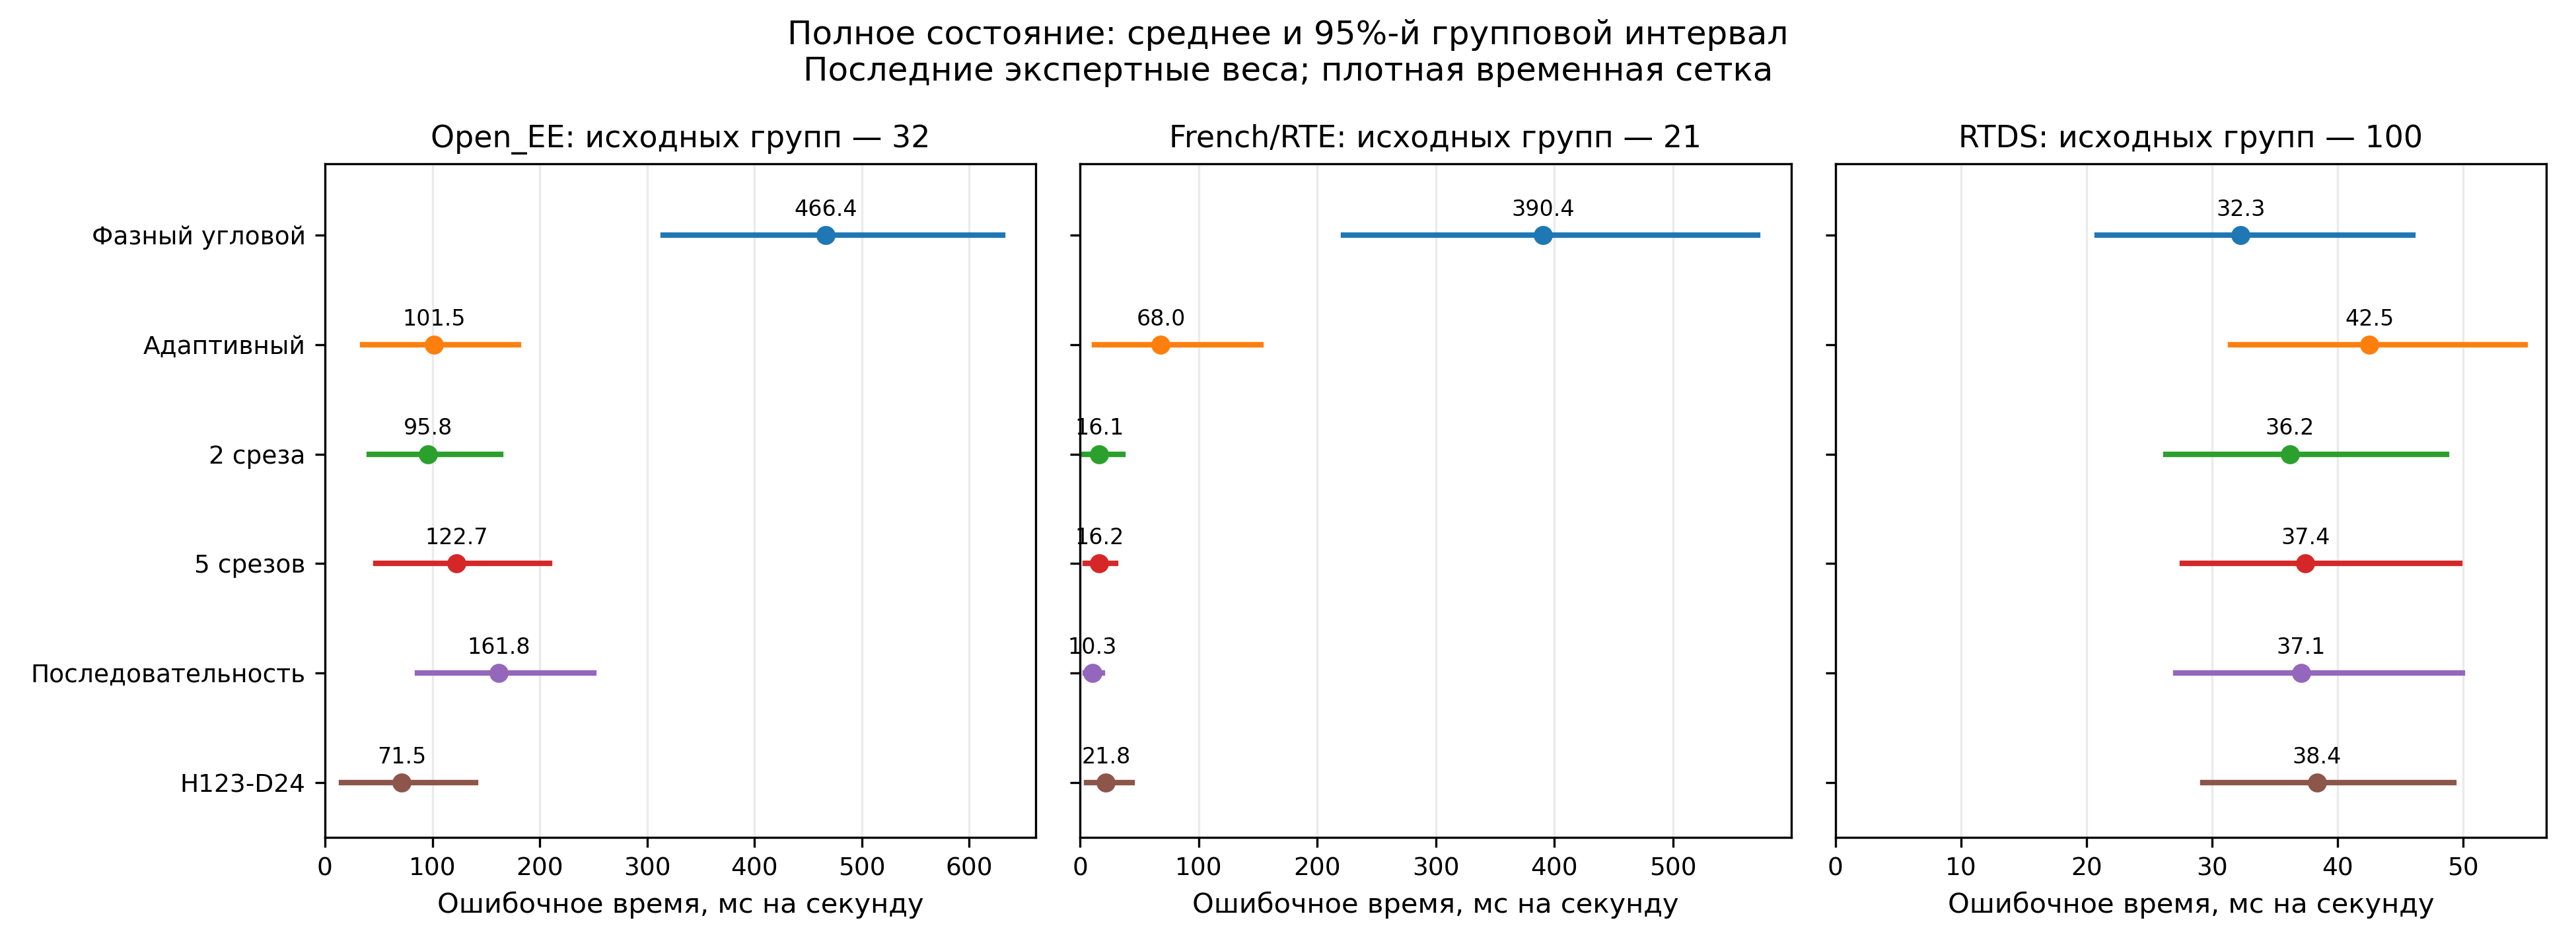
\includegraphics[width=\textwidth]{figures/ch05/ch05_engineering_error_time_article.png}
\caption{Среднее ошибочное время полного состояния
и 95\%-е интервалы по исходным группам.
Сети представлены последними экспертными весами,
масштабы осей трёх источников различаются}
\label{fig:ch5_engineering_error_time}
\figurereview{Исходный рисунок 12 статьи 5.
RTDS использует завершённый снимок разметки, который автор
ещё перепроверяет. Для печати увеличить подписи,
при необходимости разнести источники на отдельные панели,
сохранив пределы осей, средние и интервалы.}
\end{figure}

\subsection{Причины общего расхождения}
\conceptsource{Статья 5, условные ошибки H123-D24 и адаптивного
органа в Open\_EE. Знаменатели не складываются.}

Общая ошибка не показывает,
на каком экспертном состоянии орган даёт неправильный ответ.
У H123-D24 в Open\_EE ложное прямое направление
занимает в среднем 8,63\% времени экспертного обратного.
Ложное обратное составляет 7,17\% времени прямого,
лишний отказ 1,91\% применимого времени.
Для адаптивного органа получены соответственно
5,17, 14,80 и 0,034\%.

Сеть имеет меньшее общее ошибочное время,
но чаще выдаёт прямое направление вместо обратного
и чаще отказывается от применимого решения.
Эти доли относятся к разным условиям и не суммируются.
Обратное направление имеется в 18 исходных группах,
прямое в 23, применимые участки в 31.
Отсутствующее состояние не получает условную нулевую ошибку
и не улучшает среднее за счёт несуществующего испытания.

Парное сравнение сохраняет одни и те же группы
для H123-D24 и адаптивного органа.
В Open\_EE разность общего ошибочного времени
составляет $-3{,}00$ процентного пункта,
95\%-й интервал простирается от $-10{,}66$ до $+3{,}05$.
Во French/RTE разность равна $-4{,}62$ пункта,
интервал от $-13{,}09$ до $+1{,}34$.
Оба интервала включают ноль.
На имеющемся числе групп наблюдаемое уменьшение среднего
не устанавливает устойчивого преимущества.
Повторный выбор групп также не характеризует
случайность нового обучения или эксплуатационную надёжность.

\subsection{Достаточность материала для проверки быстродействия}
\conceptsource{Статья 5, конец подраздела 9.9.
Все переходы и удержание учитываются по правилам раздела 5.6.}

В экспертной части Open\_EE имеется
11 переходов из обратного направления в прямое
и девять противоположных.
Во French/RTE их соответственно один и три.
При сроке начала ответа 20~мс и удержании 5~мс
H123-D24 воспроизводит 8 из 11 и 7 из 9
переходов Open\_EE.
Адаптивный орган воспроизводит 8 из 11 и 5 из 9.
Эти числа полезны для выбора отдельных осциллограмм
и физического разбора реакции,
но слишком малы для общего вывода о быстродействии.

Наличие неприменимых отсчётов во всех исходных группах
также не означает большого числа независимых
и достаточно длинных эпизодов неприменимости.
Значительная часть соответствующих экспертных состояний
длится менее 5~мс.
Для последовательного испытания временной реакции
поэтому нужен дополнительный набор заданных режимов.
Далее рассматривается такая проверка
на программе испытаний БАВР.
